\documentclass{article}
\usepackage[utf8]{inputenc}
\usepackage[normalem]{ulem}
\usepackage{listings}

\usepackage{hyperref}
\hypersetup{
    colorlinks=true,
    linkcolor=red,
    filecolor=magenta,      
    urlcolor=cyan,
}
\usepackage{graphicx}
\usepackage{amsmath}
\usepackage{amsfonts}
\usepackage{amssymb}
\usepackage{array}
\usepackage{float}
\restylefloat{table}
%fancy headers
\usepackage{fancyhdr}
\pagestyle{fancy}
\fancyhf{}
\lhead{ICSI 401 Homework 3}
\rhead{\thepage}

\author{James Oswald}
\date{October 27, 2020}
\title{ICSI 401 Homework 3}

\begin{document}
\maketitle
\thispagestyle{fancy}
\addtocounter{section}{3}
\subsection{More root finding and related topics}
\begin{itemize}
    \item This question will test your understanding of the intermediate value theorem, which you will recall is the theorem that motivates bisection search. Consider the following function $f(x)$:
    \[f(x) = \begin{cases} x & x< -1/2 \\ x + 2 & x\geq-1/2 \end{cases}\]
    (This notation is standard and means that $f(x) = x$ whenever $x < −1/2$ and $f(x) = x + 2$ whenever $x > −1/2$.) Note that $f(x)$ is defined for every real $x$, but it has no roots. That is, there is no $x_*$ such that $f(x_*) = 0$. Nonetheless, we can find an interval $[a, b]$ such that $f(a) < 0 < f(b)$: just choose $a = -1$, $b = 1$. Why can’t we use the intermediate value theorem to conclude that f has a zero in the interval $[−1, 1]$?\newline
    
    the Intermediate Value Theorem which states that if $f$ is a continuous function on the interval $[a, b]$ and $u$ is a number between $f(a)$ and $f(b)$ then $\exists c \in (a, b): f(c) = u$. Despite the fact that we can pick $a = -1$, $b = 1$ and satisfy $f(a) < 0 < f(b)$ if we want $u = 0$, we fail to satisfy the other condition for applying the intermediate value theorem, that being that $f$ must be a continuous function on the interval $[a, b]$. This is because there is a clear gap in $f$ at $-1/2$ and due to this we can not select an interval such that we could have our desired $u = 0$ and have $f$ be continuous. 
    
    \newpage
    \item This question will test your understanding of the limitations of bisection search and Newton’s method. Consider the function $f(x) = \frac{1}{2}|x|$.
    \begin{itemize}
        \item[--] Can we use bisection search to find one of its roots? Why or why not?
        \newline\newline
        No, The Bisection Search Convergence Theorem\footnote{Couldn't find an official name  for this theorem. It's stated informally without a name on page 75 of the textbook so I just stole the name of Newton's Method Convergence Theorem and applied it here.} states that bisection search will converge to a root of $f$ in the interval $[a, b]$ iff $f$ is a continuous function and $f(a)$ and $f(b)$ have opposite signs. While we can easily show $\frac{1}{2}|x|$ is continuous, it is clear that we can never satisfy the second condition since $f(x)$ will never be negative due it taking the absolute value x and scaling it by a positive factor, always resulting in a positive number. Thus $f(a)$ and $f(b)$ can never have opposite signs for any $a, b$ we select, and therefore since we fail to satisfy the bisection search convergence theorem we can't use bisection search to find a root of $f$.
        \newline\newline
        \item[--] Can we use Newton’s method to find one of its roots? Why or why not?
        \newline\newline
        Yes, In this case we won't use The Newtons Converge Method Theorem since we the second derivative of $f$ is not continuous at 0. Instead we will show numerically that the first iteration of newtons method for this particular $f$ will always solve for the root for any $x_0$ we pick as long as we don't pick the root itself as our starting point since $f'(0)$ will be undefined.
        \begin{equation}
        \begin{aligned}
            f(x) = \frac{1}{2}|x| = \begin{cases} \frac{1}{2}x & x \geq 0 \\ -\frac{1}{2}x & x<0 \end{cases} & \quad \textrm{and} & f'(x) = \begin{cases} \frac{1}{2} & x > 0 \\ -\frac{1}{2} & x<0 \end{cases}
        \end{aligned}
        \end{equation}
        Newtons method states that $x_1$ will be a better approximation, but we will see that by calculating it for this $f$, it will have converged to the root itself.
        \begin{equation}
        \begin{aligned}
           x_1 = x_0 - \frac{f(x_0)}{f'(x_0)} = \begin{cases} x_0 - \frac{\frac{1}{2}x_0}{\frac{1}{2}} & x_0 > 0 \\ x_0 - \frac{-\frac{1}{2}x_0}{-\frac{1}{2}} & x_0 < 0 \end{cases} = x_0 - x_0 = 0 
        \end{aligned}
        \end{equation}
        the jump from the piecewise formulation to 0 is only legal if we choose $x_0$ not to be 0 itself which is perfectly legal. Thus newtons method will always converge to the root of $f$, 0, after its first iteration. 
    \end{itemize}
\end{itemize}

\newpage
\subsection{Fixed point iteration}
\begin{itemize}
    \item Complete problem 4.7.12 in the textbook. This will test your knowledge of what a fixed point of a function is, how to find them, and how to determine when iteration will converge to a fixed point.
    \newline
    12. Let function $\varphi(x) = (x^2 + 4) / 5$  
    \begin{itemize}
        \item[(a)] Find the fixed point(s) of $\varphi(x)$.
        \newline \newline
        Since our $\varphi(x)$ is simple we can easily compute this algebraically with $x = \varphi(x)$
        \begin{equation}
        \begin{split}
            x &= \varphi(x) \\
            x &= (x^2 + 4) / 5 \\
            5x &= x^2 + 4 \\
            0 &= x^2 - 5x + 4 \\
            0 &= (x - 1)(x - 4) \\
            x &= 1 \quad \textrm{or} \quad x = 4 \\
        \end{split}
        \end{equation}
        Thus we see that our fixed points of $\varphi(x)$ are 0 and 4.
        \newline
        \item[(b)] Would the fixed point iteration, $x_{k+1} = \varphi(x_k)$, converge to a fixed point in the interval $[0,2]$ for all initial guesses $x_0 \in [0, 2]$?
        \newline\newline
        The fixed point convergence theorem states that if $\varphi(x)$ is continuous and $|\varphi'(x)| < 1$ (the function is a contraction) on a range $[a, b]$ centered around a fixed point $x_*$ then fixed point iteration will converge to $x_*$. In our case we know $\varphi(x)$ is continuous on the interval $[0, 2]$ centered around what we believe to be a fixed point at 1. Now all we need to do is prove $\varphi(x)$ is also a contraction on this interval as well. We begin by calculating the derivative of $\varphi(x)$,
        \begin{equation}
        \begin{split}
            \varphi(x) = (x^2 + 4) / 5 = \frac{x^2}{5} + \frac{4}{5} \quad \textrm{and} \quad
            \varphi'(x) = \frac{2}{5}x 
        \end{split}
        \end{equation}
        \newline
        Since $\frac{2}{5}x$ is a line with a positive slope we know its maximum in the range $[0, 2]$ will be its left endpoint $2$ and its minimum will be its right endpoint $0$. Since we're applying absolute value on this, the min might be greater then the max but this means if neither the max nor min are over 1, then we've proved its a contraction.
        \begin{equation}
        \begin{split}
            |\varphi'(0)| = \left|\frac{2}{5}(0)\right| = 0 < 1 \quad \textrm{and} \quad |\varphi'(2)| = \left|\frac{2}{5}(2)\right| = 4/5 < 1
        \end{split}
        \end{equation}
        Thus we've proved $\varphi(x)$ is a contraction on $[0, 2]$ and with that proved we satisfy The fixed point convergence theorem. $\varphi(x)$ is guaranteed to converge to a fixed point within this range. 
    \end{itemize}
    
    \newpage
    \item Application question. Here’s how this works: You get full points for a reasonable attempt. So you MUST attempt this question. You get extra credit if you’re correct. This question presents a simple model of population dynamics, and analyzes its equilibrium states. Models like this, but more complicated, can be used to predict global population trends, for instance. \newline 
    Let $N_t$ denote the number of individuals in a population at time $t$. We will assume that $N_t$ evolves at each time step according to the following equation:
    \[N_{t+1} = N_t + rN_t(1 - N_t/K)\]
    where
    \begin{itemize}
        \item[--] $r$ is the birth minus death rate (per existing individual) parameter. Let us assume that it is larger than 0.
        \item[--] $K$ is a positive constant representing fundamental resource limitations for the population. For example, on Earth, there is only a finite amount of of consumable biomass, and so the number of humans on Earth probably cannot grow to infinity. Note that when $N_t > K$, we have $N_{t+1} − N_t < 0$.
    \end{itemize}
    Supposing we start with some initial population $N_0$, we can calculate $N_t$ as follows:
    \begin{itemize}
        \item[--] Define $F(x) = x + rx(1 - x/K)$.
        \item[--] Define $x = N_0$.
        \item[--] Compute $N_t = F \circ F \circ ... \circ F(x)$, where $F$ is applied $t$ times
    \end{itemize}
    Now, we want to determine cases where this process converges. Suppose $r > 0$ and $K > 0$ are fixed.
    \begin{itemize}
    
        \newpage
        \item[--] \textbf{Determine all non-negative values of $x$ for which $F$ is a contraction.} Hints: Recall that we say that a function $F$ is a contraction if its Lipschitz constant $L$ is strictly less than 1. In other words:
        \[|F(z) - F(z')| \leq L \cdot |z - z'|\]
        for all $z, z' > 0$. Remember that you can get an upper bound on $L$ by upper bounding $|F'(z)|$ for every $z$.\newline You should get an answer of the form "$x > g(K)$" for some explicit function $g$ that you have to determine.
        \newline\newline
        We begin by determining $F'(x)$ so that we may calculate when x is a contraction. The easiest way to do this is to first convert $F$ to a nice easy to differentiate polynomial. 
        \begin{equation}
        \begin{split}
            F(x) &= x + rx(1 - x/K) = x + rx - \frac{r}{K}x^2 = \frac{-r}{K}x^2 + rx + x \\
            F'(x) &= \frac{-2r}{K}x + r + 1
        \end{split}
        \end{equation}
        We use $F'(x)$ to solve for where x is a contraction and get an answer with respect to $K$. Despite an hour of work I'm stuck generalizing this result to  the interval $(g(K), \infty)$ using the definition of contraction provided in the hint. 
        \begin{equation}
        \begin{split}
             |F'(x)| &< 1 \\
            \left|\frac{-2r}{K}x + r + 1\right| &< 1 \\
            -1 < \frac{-2r}{K}x + r + 1 &< 1 \\
            -r-2 < \frac{-2r}{K}x &< -r \\
            -Kr - 2K < -2rx &< -Kr \\
            \frac{-Kr}{-2r} + \frac{-2K}{-2r} > x &> \frac{-Kr}{-2r} \\
           \frac{1}{2}K + \frac{K}{r} > x &> \frac{1}{2}K
        \end{split}
        \end{equation}
        
        \newpage
        \item[--] Suppose that $x \leq K$. Show that $F(x) \geq x$.
        \newline\newline
        I begin by deriving an equivalent statement for $F(x) \geq x$ which is trivial to prove.
        \begin{equation}
        \begin{split}
            F(x) &\geq x \\
            x + rx(1 - x/K) &\geq x \\
            rx(1-x/K) &\geq 0 \\
            1-x/K &\geq 0 \\
            x/K &\leq 1
        \end{split}
        \end{equation}
        Since $x \leq K$ it should be immediately obvious that $x/K \leq 1$ is true since the numerator is smaller then or equal to the denominator. Thus $x \leq K \Rightarrow F(x) \geq x$
        \newline
        \item[--] Suppose that $x > K$. Show that $F(x) < x$.
        \newline\newline
        This is done via the exact same proof process as the last problem. I begin by deriving an equivalent statement for $F(x) < x$ which is trivial to prove.
        \begin{equation}
        \begin{split}
            F(x) &< x \\
            x + rx(1 - x/K) &< x \\
            rx(1-x/K) &< 0 \\
            1-x/K &< 0 \\
            x/K &> 1
        \end{split}
        \end{equation}
        Since $x > K$ it should be immediately obvious that $x/K > 1$ is true since the denominator is larger then the numerator. Thus $x > K \Rightarrow F(x) < x$
        \newline
        \item[--] What we've shown, then, is that $F$ is a contraction on the interval $(g(K), \infty)$, and, furthermore, if we fix any $L > g(K), U > K > L$, then $F$ maps any value $y \in [L, U]$ to some value $F(y) \in [L, U]$. Thus, by Banach’s fixed point theorem, we can conclude that $F$ has a unique fixed point $x_*$ in the interval $[L, U]$, and iterated application of $F$ converges to $x_*$. Here, $x_*$ is the limiting population size! \newline
        Furthermore, since $K$ is guaranteed to be in $[L, U]$, we see that $x_* = K$. That is, if we start at any positive population size $> g(K)$, the population will eventually converge to $K$ (in fact, with more work, one can show that this happens for any positive initial population size). This makes intuitive sense: remember that $K$ represents the resource constraints on the population, so this says that the population will converge to the capacity of its environment.
    \end{itemize}
\end{itemize}

\newpage
\subsection{Condition numbers and algorithmic stability}
Recall that the relative condition number $\kappa(x)$ of a function $f(x)$ is approximately the factor by which a relative error in the input gets magnified in the relative error in the output. I.e., if $x$ is perturbed to $\hat{x}$, then
\[\left|\frac{f(x)-f(\hat{x})}{f(x)}\right|\approx\kappa(x)\left|\frac{x - \hat{x}}{x}\right|\]
We gave a formula for $\kappa(x)$ in class, and it also appears in the textbook.
\begin{itemize}
    \item Qualitatively speaking, if the relative condition number of a function is large, does this make the function ill-conditioned, or well-conditioned (choose one)?
    \newline\newline
    By definition, a large relative condition number means that a function is ill-conditioned.
    \item Suppose that a problem has a very small condition number for a given input, but the relative error of the output of an algorithm for the problem is large. Is this the fault of the problem or of the algorithm (choose one)?
    \newline\newline
    This would be a fault of the algorithm since the relative condition number is small, meaning we expect the problem to be well-conditioned and not have a large relative error.
    \item Complete problem 6.3.5 on compound interest in the textbook, and make sure that you understand how they derived $\mathcal{I}_n(x)$. Also, note that\newline $\lim_{n\to\infty} \mathcal{I}_n(x) = e^x$. For part (d), demonstrate your method in Matlab. \newline\newline
    (Not going to copy the problem down into this document since its very large)
    \begin{itemize}
        \item[(a)] 
        We can begin our calculation by obtaining the derivative of $\mathcal{I}_n$ with respect to $x$ which we will use to calculate the relative condition number of the problem $\kappa_{\mathcal{I}_n}(x)$.
        \[\mathcal{I}_n(x) = \left(1 + \frac{x}{n}\right)^n \quad \textrm{and} \quad \mathcal{I}_n'(x) = n(x + n)^{-1}\left(1 + \frac{x}{n}\right)^n \]
        \[\kappa_{\mathcal{I}_n}(x) = \left|\frac{x \cdot \mathcal{I}_n'(x)}{\mathcal{I}_n(x)} \right| = \left|\frac{x \cdot n(x + n)^{-1}\left(1 + \frac{x}{n}\right)^n}{\left(1 + \frac{x}{n}\right)^n} \right| = \left|\frac{nx}{x+n}\right|\] 
        for $x = 5$, $\kappa_{\mathcal{I}_n}(0.5) = \left|\frac{0.5n}{n + 0.5}\right|$. This is very well-conditioned, looking at a graph of it we see the relative condition number stays relatively small, we prove it stays this way by taking the limit of it with respect to $n$ we see $\lim_{n\to\infty}\mathcal{I}_n(0.5) = 0.5$ meaning that our relative condition number will never be over 0.5, staying small, which means the problem is well-conditioned.
        
        \newpage
        \item[(b)] (the MATLAB file has also been attached: hw33b.m)
        \newline
        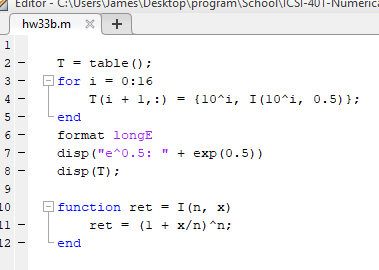
\includegraphics[scale=0.4]{Homework3/3.3b.png}
        \newline
        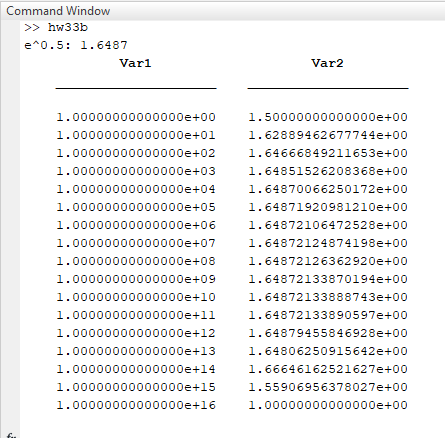
\includegraphics[scale=0.4]{Homework3/res3.3b.png}
        \item[(c)] The results begin converging to the right answer but then suddenly begin shifting away at $n=8$. My hypothesis is that when $n$ gets very large, the $x/n$ term approaches 0. Since there are only so many representable floating point numbers, the smaller the $x/n$ gets, the less accurate it is which is why we start shifting away and then, finally at $10^16$ for me, it gets so small that it is forced to store this term as 0. thus $z^n = (1 + 0)^n = 1$ and I is computed as 1, when in real life the really small $x/n$ term would be be brought back to get the right answer when preforming the exponentiation with $n$. As previously computed, the relative condition number of this problem is at most 0.5, which is more then the error we are getting here.  
        
        \newpage
        \item[(d)] Yes, a better solution would be to analyze at what $n$ the $\mathcal{I}_n(0.5)$ begins to diverge from what we know to be the correct limit. At that point hard set $\mathcal{I}_n(0.5)$ to return the correct limit, $e^{0.5}$. \newline\newline
        (the MATLAB file has also been attached: hw33d.m)
        \newline
        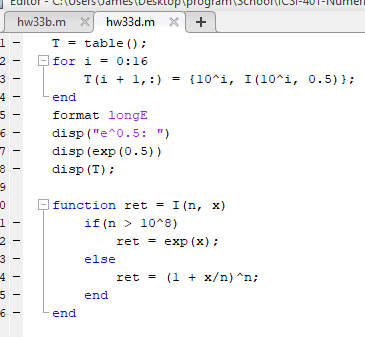
\includegraphics[scale=0.4]{Homework3/3.3d.png}
        \newline
        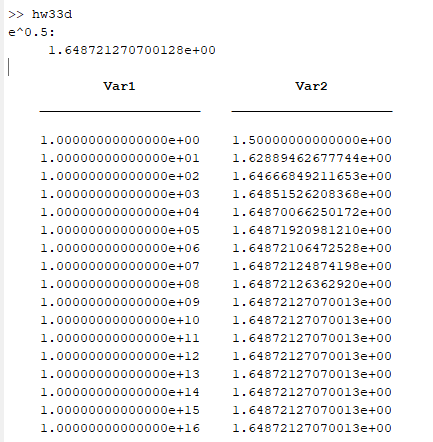
\includegraphics[scale=0.4]{Homework3/res3.3d.png}
        \newline
        We can see from the results that this works much better for computing with large $n$s by avoiding the issues caused by floating point representation entirely and instead favoring our knowlege of the limit. 
    \end{itemize}
\end{itemize}

\newpage
\subsection{Some numerical linear algebra}
\begin{itemize}
    \item This problem will teach you how to work with the LU decomposition of a matrix programmatically to solve a linear system. The Matlab function lu(A) returns [L, U, P], where L is a lower triangular matrix, U is an upper triangular matrix, and P is a permutation matrix, such that
    \[A = P^TLU\]
    Complete the following code to produce a solution to the equation A$x = b$, without multiplying the input matrices.
    \begin{lstlisting}[language=MATLAB]
function x = solve_with_LU(L, U, P, b)
%
% Given a lower triangular matrix L, an upper triangular matrix U,
% a permutation matrix P, and a vector b,
% return a solution to the equation P'LUx = b.
%
    z = P'\b;
    y = L\z;
    x = U\y;
end
    \end{lstlisting}
    \newline
    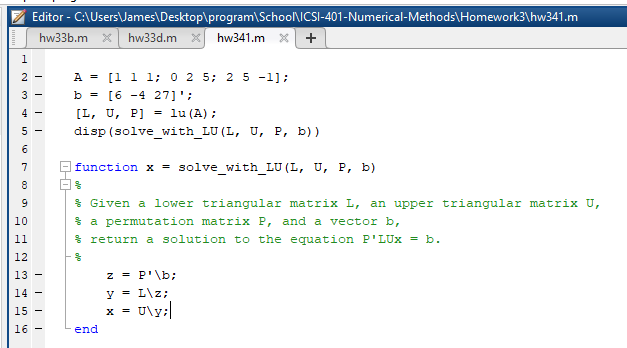
\includegraphics[scale=0.4]{Homework3/3.4.1.png}
    \newline
    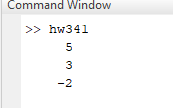
\includegraphics[scale=0.4]{Homework3/res3.4.1.png}
    \newline
    To make sure I got the right answer, I also use my matrix calculator to compute the answer the traditional way and make sure they match. 
    \newline
    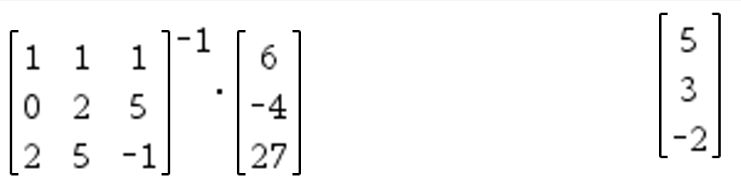
\includegraphics[scale=0.4]{Homework3/trad3.4.1.png}
    \newline
    
    \newpage
    \item In Matlab, compute the matrices P, L, and U from the LU decomposition of the matrix
    \[A = \begin{pmatrix}10^{-20} & 1 \\ 1 & 1 \end{pmatrix}\]
    and use the completed function above to obtain the solution to the system A$x = b$, where
    \[b = \begin{pmatrix}1 \\ 1 \end{pmatrix}\] Please note that you have to turn in Matlab code for this question, including the completed version of the function above.
    \newline\newline
    I use the code from the previous problem for my computation, however it seems that the high precision of $10^{-20}$ is just interpreted as a 0 during the computation with the lower triangular, giving an approximately correct result.   
    \newline\newline
    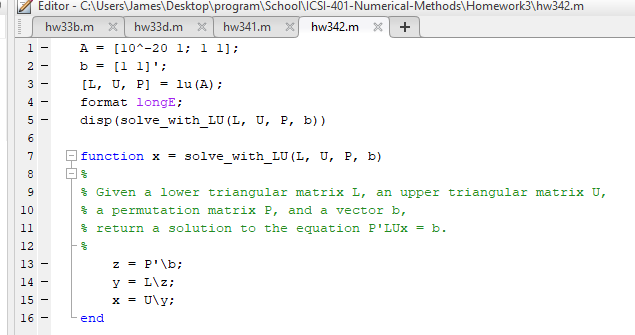
\includegraphics[scale=0.4]{Homework3/3.4.2.png}
    \newline
    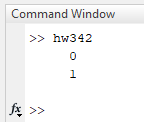
\includegraphics[scale=0.4]{Homework3/res3.4.2.png}
    \newline
\end{itemize}

Note: code for 3.4 can be found in the attached files hw341.m and hw342.m


\end{document}